\documentclass[review]{siamart1116}

%% ------------------------------------------------------------------
%% Code used in examples, needed to reproduce 
%% ------------------------------------------------------------------
%% Used for \set, used in an example below
\usepackage{braket,amsfonts}

%% Used in table example below
\usepackage{array}

%% Used in table and figure examples below
\usepackage[caption=false]{subfig}
%% Used for papers with subtables created with the subfig package
\captionsetup[subtable]{position=bottom}
\captionsetup[table]{position=bottom}

%% Used for PgfPlots example, shown in the "Figures" section below.
\usepackage{pgfplots}

%% Used for creating new theorems, remarks
\newsiamthm{claim}{Claim}
\newsiamremark{rem}{Remark}
\newsiamremark{expl}{Example}
\newsiamremark{hypothesis}{Hypothesis}
\crefname{hypothesis}{Hypothesis}{Hypotheses}

%% Algorithm style, could alternatively use algpseudocode
\usepackage{algorithmic}

%% For figures
\usepackage{graphicx,epstopdf}


%% For referencing line numbers
\Crefname{ALC@unique}{Line}{Lines}

%% For creating math operators
\usepackage{amsopn}
\DeclareMathOperator{\Range}{Range}

%strongly recommended
\numberwithin{theorem}{section}

%% ------------------------------------------------------------------
%% Macros for in-document examples. These are not meant to reused for
%% SIAM journal papers.
%% ------------------------------------------------------------------
\usepackage{xspace}
\usepackage{bold-extra}
\usepackage[most]{tcolorbox}
\newcommand{\BibTeX}{{\scshape Bib}\TeX\xspace}
\newcounter{example}
\colorlet{texcscolor}{blue!50!black}
\colorlet{texemcolor}{red!70!black}
\colorlet{texpreamble}{red!70!black}
\colorlet{codebackground}{black!25!white!25}

% additional useful packages
\usepackage[disable]{todonotes}
%\usepackage{showlabels}

\newcommand\bs{\symbol{'134}} % print backslash in typewriter OT1/T1
\newcommand{\preamble}[2][\small]{\textcolor{texpreamble}{#1\texttt{#2 \emph{\% <- Preamble}}}}

\lstdefinestyle{siamlatex}{%
  style=tcblatex,
  texcsstyle=*\color{texcscolor},
  texcsstyle=[2]\color{texemcolor},
  keywordstyle=[2]\color{texemcolor},
  moretexcs={cref,Cref,maketitle,mathcal,text,headers,email,url},
}

\tcbset{%
  colframe=black!75!white!75,
  coltitle=white,
  colback=codebackground, % bottom/left side
  colbacklower=white, % top/right side
  fonttitle=\bfseries,
  arc=0pt,outer arc=0pt,
  top=1pt,bottom=1pt,left=1mm,right=1mm,middle=1mm,boxsep=1mm,
  leftrule=0.3mm,rightrule=0.3mm,toprule=0.3mm,bottomrule=0.3mm,
  listing options={style=siamlatex}
}

\newtcblisting[use counter=example]{example}[2][]{%
  title={Example~\thetcbcounter: #2},#1}

\newtcbinputlisting[use counter=example]{\examplefile}[3][]{%
  title={Example~\thetcbcounter: #2},listing file={#3},#1}

\DeclareTotalTCBox{\code}{ v O{} }
{ %fontupper=\ttfamily\color{texemcolor},
  fontupper=\ttfamily\color{black},
  nobeforeafter,
  tcbox raise base,
  colback=codebackground,colframe=white,
  top=0pt,bottom=0pt,left=0mm,right=0mm,
  leftrule=0pt,rightrule=0pt,toprule=0mm,bottomrule=0mm,
  boxsep=0.5mm,
  #2}{#1}

% Stretch the pages
\patchcmd\newpage{\vfil}{}{}{}
\flushbottom

%% ------------------------------------------------------------------
%% End of macros for in-document examples. 
%% ------------------------------------------------------------------

%% ------------------------------------------------------------------
%% HEADING INFORMATION
%% ------------------------------------------------------------------
\begin{tcbverbatimwrite}{tmp_\jobname_header.tex}
\title{Sympletic Model-Reduction with a Weighted Inner Product%
  \thanks{%
\funding{Ashish Bhatt and Bernard Haasdonk gratefully acknowledges the support of DFG grant number HA5821/5-1.}} }

\author{Babak Maboudi Afkham%
  \thanks{Institute of Mathematics (MATH), School of Basic Sciences (FSB), Ecole Polytechnique F\'ed\'erale de Lausanne, 1015 Lausanne, Switzerland (\email{babak.maboudi@epfl.ch}, \email{jan.hesthaven@epfl.ch}).}%
  \and
  Ashish Bhatt%
  \thanks{University of Stuttgart, IANS, Pfaffenwaldring 57, 70569 Stuttgart, Germany (\email{[ashish.bhatt,haasdonk]@mathematik.uni-stuttgart.de}).}
  \and
  Bernard Haasdonk%
  \footnotemark[3]
  \and
  Jan S. Hesthaven%
  \footnotemark[2]
}

% Custom SIAM macro to insert headers
\headers{Sympletic Model-Reduction with a Weighted Inner Product}
{B. M. Afkham, A. Bhatt, B. Haasdonk, and J. S. Hesthaven}
\end{tcbverbatimwrite}
\input{tmp_\jobname_header.tex}

% Optional: Set up PDF title and authors
\ifpdf
\hypersetup{ pdftitle={Guide to Using  SIAM'S \LaTeX\ Style} }
\fi

%% ------------------------------------------------------------------
%% END HEADING INFORMATION
%% ------------------------------------------------------------------

%% ------------------------------------------------------------------
%% MAIN Document
%% ------------------------------------------------------------------
\begin{document}
\maketitle

%% ------------------------------------------------------------------
%% ABSTRACT
%% ------------------------------------------------------------------
\begin{tcbverbatimwrite}{tmp_\jobname_abstract.tex}
\begin{abstract}
In the recent years, a considerable attention has been geared toward preserving structures and invariants in reduced basis methods, to enhance the stability and the robustness of the reduced system. In the context of Hamiltonian systems, symplectic model reduction is an approach that tends to construct a reduced order system that preserve the symplectic symmetry of Hamiltonian systems. However, the symplectic methods are based on the standard Euclidean inner products and are not suitable for problems that are equipped with a more general inner product. In this paper we generalize the symplectic model reduction method such that it can adapt to the norms and the inner products most appropriate to the problem while preserving the symplectic symmetry of Hamiltonian systems. To construct a reduced basis and accelerate evaluation of nonlinear terms, a greedy generation of a symplectic basis is proposed. Furthermore, it is shown that the greedy approach yields a norm bounded reduced basis. The efficiency, accuracy, and stability of this model reduction technique is illustrated through the simulations of a vibrating elastic beam and the sine-Gordon equation.
\end{abstract}

\begin{keywords}
Weighted structure-preserving MOR, Hamiltonian system, Greedy reduced basis, Symplectic DEIM
\end{keywords}

\begin{AMS}
78M34, 34C20, 35B30, 37K05, 65P10, 37J25
\end{AMS}
\end{tcbverbatimwrite}
\input{tmp_\jobname_abstract.tex}
%% ------------------------------------------------------------------
%% END HEADER
%% ------------------------------------------------------------------

%% ------------------------------------------------------------------
%% MAIN Body
%% ------------------------------------------------------------------

\section{Introduction}
\label{sec:intro}

Reduced order models have emerged as a powerful approach to cope with increasingly complex new applications in engineering and science. These methods substantially reduce the dimensionality of the problem by constructing a reduced configuration space. Exploration of the reduced space is then possible with significant acceleration \cite{hesthaven2015certified,Haasdonk2017}.

Over the past decade, reduced basis (RB) methods have demonstrated great success in lowering of the computational costs of solving elliptic and parabolic differential equations \cite{ito1998reduced,ito2001reduced}. However, model order reduction (MOR) of hyperbolic problems remains a challenge. Such problems often arise from a set of conservation laws and invariants. These intrinsic structures are lost during MOR which results in a qualitatively wrong, and sometimes unstable reduced system \cite{Amsallem:2014ef}.

%To have a sense of this error, error estimation is important from applications point of view \cite{HaasdonkOhlberger11,RuinerEtAl12,BhattEtAl18}. But it can difficult and expensive to compute useful error bounds. When one is interested in a cheap surrogate for the error incurred or when the conserved quantity is an output of the system, it becomes imperative to preserve this structure through model order reduction.

Recently, the construction of RB methods that conserve intrinsic structures has attracted attention \cite{doi:10.1137/17M1111991,1705.00498,kalashnikova2014stabilization,farhat2015structure,doi:10.1137/110836742,doi:10.1137/140959602,beattie2011structure,doi:10.1137/140978922}. Structure preservation in MOR not only constructs a physically meaningful reduced system, but can also enhance the robustness and stability of the reduced system. In system theory, conservation of passivity can be found in the work of \cite{polyuga2010structure,gugercin2012structure}. Energy preserving and inf-sup stable methods for finite element methods (FEM) are developed in \cite{farhat2015structure,ballarin2015supremizer}. Also, a conservative MOR technique for finite-volume methods is proposed in \cite{1711.11550}.

Moreover, the simulation of reduced models incurs solution errors and the estimation of this error is essential in applications of MOR \cite{HaasdonkOhlberger11,RuinerEtAl12,BhattEtAl18}. Finding tight error bounds for a general reduced system has shown to be computationally expensive and often impractical. Therefore, when one is interested in a cheap surrogate for the error or when the conserved quantity is an output of the system, it becomes imperative to preserve system structures in the reduced model.

In the context of Lagrangian and Hamiltonian systems, recent works provide a promising approach to the construction of robust and stable reduced systems. Carlberg, Tuminaro, and Boggs \cite{doi:10.1137/140959602} suggest that a reduced order model of a Lagrangian system be identified by an approximate Lagrangian on a reduced order configuration space. This allows the reduced system to inherit the geometric structure of the original system. A similar approach has been adopted in the work of Peng and Mohseni \cite{doi:10.1137/140978922} and in the work of Maboudi Afkham and Hesthaven \cite{doi:10.1137/17M1111991} for Hamiltonian systems. They construct a low-order symplectic linear vector space, i.e. a vector space equipped with a symplectic 2-form, as the reduced space. Once the symplectic reduced space is generated, a symplectic projection result in a physically meaningful reduced system. A proper time-stepping scheme then preserves the Hamiltonian structure of the reduced system. It is shown in \cite{doi:10.1137/17M1111991,doi:10.1137/140978922} that this approach preserves the overall dynamics of the original system and enhances the stability of the reduced system. Despite the success of these method in MOR of Hamiltonian systems, these techniques are only compatible with the Euclidean inner product. Therefore, the computational structures that arise from a natural inner product of a problem will be lost during MOR.

Weak formulations and inner-products, defined on a Hilbert space, are at the core of the error analysis of many numerical methods for solving partial differential equations. Therefore, it is natural to seek MOR methods that consider such features. At the discrete level, these features often require a Euclidean vector space to be equipped with a generalized inner product, associated with a weight matrix $X$. Many works enabled conventional MOR techniques compatible with such inner products \cite{sen2006natural}. However, a MOR method that simultaneously preserves the symplectic symmetry of Hamiltonian systems remains unknown. 

In this paper, we seek to combine a classical MOR method with respect to a weight matrix with the symplectic MOR. Generalized inner products often require a state transformation to a non-canonical coordinate system. This restricts the choices of symplectic integrators that can be used in a numerical integration of the reduced system. The reduced system constructed by the new method, however, is a Hamiltonian system on a symplectic linear vector space with a canonical coordinate system. Therefore, any symplectic integrator can ensure long-time and robust numerical integration. It is demonstrated that the new method can be viewed as the natural extension to \cite{doi:10.1137/17M1111991}, and therefore retains the structure preserving features, e.g. symplecticity and stability. We also present a greedy approach for the construction of a generalized symplectic basis for the reduced system. Symplectic bases are often non-orthogonal and therefore not norm bounded. However, we show that the condition number of the basis generated by the greedy method is bounded by the condition number of the weight matrix $X$. Finally, to accelerate the evaluation of nonlinear terms in the reduced system, we present a variation of the discrete empirical interpolation method (DEIM) that preserves the symplectic structure of the reduced system.

What remains of this paper is organized as follows. In \cref{sec:hamil} we cover the required background on the Hamiltonian and the generalized Hamiltonian systems. \Cref{sec:mor} summarizes classic MOR routine with respect to a weighted norm and the symplectic MOR method with respect to the standard Euclidean inner product. We introduce the symplectic MOR method with respect to a weighted inner product in \cref{sec:normmor}. \Cref{sec:res} illustrates the performance of the new method through a vibrating beam and the sine-Gordon equation. We offer a few conclusive remarks in \cref{sec:conc}.

\section{Hamiltonian Systems}
\label{sec:hamil}

In this section we discuss the basic concepts around the geometry of symplectic linear vector spaces and introduce Hamiltonian and Generalized Hamiltonian systems.

\subsection{Generalized Hamiltonian Systems}
\label{sec:hamil.1}

Let $(\mathbb R^{2n}, \Omega)$ be a symplectic linear vector space, with $\mathbb R^{2n}$ the configuration space and $\Omega:\mathbb R^{2n}\times\mathbb R^{2n} \to \mathbb R$ a closed, skew-symmetric and non-degenerate 2-form on $\mathbb R^{2n}$. Given a smooth Hamiltonian function $H:\mathbb R^{2n} \to \mathbb R$, the \emph{generalized Hamiltonian} equation of evolution reads
\begin{equation} \label{eq:hamil.1}
\left\{
\begin{aligned}
	& \dot z = J_{2n} \nabla_z H,  \\
	&  z(0) = z_0.
\end{aligned}
\right.
\end{equation}
Here $z\in \mathbb R^{2n}$ is the configuration coordinates and $J_{2n}$ is a full-rank and skew-symmetric $2n\times 2n$ matrix such that $\Omega(x,y) = x^TJ_{2n}y$, for all state vectors $x,y\in \mathbb R^{2n}$ \cite{Marsden:2010:IMS:1965128}. Note that one can Always find a coordinate transformation $\tilde z = V z$, with $V \in \mathbb R^{2n\times 2n}$ such that $J_{2n}$ takes the form $\mathbb{J}_{2n}$ in the new coordinate system \cite{de2006symplectic}, and $\mathbb{J}_{2n}$ is the standard symplectic matrix given as
\begin{equation} \label{eq:hamil.2}
	\mathbb{J}_{2n} = 
	\begin{pmatrix}
	0_n & I_n \\
	-I_n & 0_n
	\end{pmatrix}.
\end{equation}
Here $0_n$ and $I_n$ are the zero matrix and the identity matrix of size $n\times n$, respectively. A central feature of Hamiltonian systems is the conservation of the Hamiltonian which we summarize in the following theorem.
\begin{theorem}
Consider the flow $\phi_t:\mathbb R \times \mathbb R^{2n} \to \mathbb R^{2n}$ of the Hamiltonian system (\ref{eq:hamil.1}). Then $H \circ \phi_t = H$.
\end{theorem}

Under a general coordinate transformation, the equations of evolution of a Hamiltonian system might not take the form (\ref{eq:hamil.1}). It turns out that only transformations which preserve the symplectic form, \emph{symplectic transformations}, also preserve the form of a Hamiltonian system. Suppose that $(\mathbb R^{2n},\Omega)$ and $(\mathbb R^{2k},\Lambda)$ are two symplectic linear vector spaces. The transformation $\alpha:\mathbb R^{2n}\to\mathbb R^{2k}$ is a symplectic transformation if
\begin{equation}
	\Omega(x,y) = \Lambda(\alpha(x),\alpha(y)), \quad \text{for all } x,y\in\mathbb R^{2n}.
\end{equation}

\section{Model order reduction}
\label{sec:mor}
Hamiltonian systems are a special case of port-Hamiltonian systems where energy of the system is bounded by the work done on the system instead of being constant. Structure-preserving reduction methods , based on POD and optimal subspaces, and hyper-reduction methods for nonlinear port-Hamiltonian systems are introduced in \cite{chaturantabut2016structure}, where they also derive a priori error bounds. The present work has similar intentions and builds on \cite{doi:10.1137/140978922,doi:10.1137/17M1111991} to hyper-reduce a Hamiltonian system in a weighted norm, which could be more attractive in certain applications.

In this section we summarize the fundamentals of MOR and discuss the conventional approach to MOR with a weighted inner product. We then recall the main results from \cite{doi:10.1137/17M1111991} regarding symplectic MOR. In \cref{sec:normmor} we shall combine the two concepts to introduce the symplectic MOR of Hamiltonian systems with respect to a weighted inner product.

\subsection{Model-reduction with a weighted inner product} \label{sec:mor.1}
Consider a dynamical system of the form
\begin{equation} \label{eq:mor.1}
\left\{
\begin{aligned}
	\dot x(t) &= f(t,x), \\
	x(0) &= x_0.
\end{aligned}
\right.
\end{equation}
where $x\in \mathbb R^{m}$ and $f:\mathbb R \times \mathbb R^{m} \to \mathbb R^{m}$ is some continuous function. In this paper we assume that the time $t$ is the only parameter on which the solution vector $x$ depends. Nevertheless, it is straightforward to generalize the findings of this paper to the case of parametric MOR, where $x$ depends on a larger set of parameters that belong to a closed and bounded subset.

Suppose that $x$ is well approximated by a low dimensional linear subspace with the basis matrix $V=[v_1|\dots|v_k]\in \mathbb R^{m\times k}$, $v_i\in \mathbb R^{m}$ for $i=1,\dots,k$. The approximate solution to (\ref{eq:mor.1}) in this basis reads
\begin{equation} \label{eq:mor.2}
	x \approx Vy,
\end{equation}
where $y \in \mathbb R^k$ are the expansion coefficients of $x$ in the basis $V$. Note that projection of $x$ onto colspan$(V)$ depends on the inner product and the norm defined on (\ref{eq:mor.1}). We define the weighted inner product
\begin{equation} \label{eq:mor.3}
	\left\langle \zeta,\eta \right\rangle_X = \zeta^TX \eta,\quad \text{for all } \zeta,\eta \in \mathbb R^m,
\end{equation}
for some symmetric and positive-definite matrix $X\in \mathbb{R}^{m\times m}$ and refer to $\|\cdot \|_X$ as the $X$-norm associated to this inner product. If we choose $V$ to be an orthonormal basis with respect to the $X$-norm ($V^TXV=I_k$), then the operator
\begin{equation} \label{eq:mor.4}
	P_{X,V}(\zeta) = VV^TX\zeta, \quad \text{for all } \zeta \in \mathbb R^{m}
\end{equation}
becomes idempotent, i.e. $P_{X,V}$ is a projection operator onto colspan$(V)$.

Now suppose that the \emph{snapshot matrix} $S=[x(t_1)|x(t_2)|\ldots|x(t_N)]$ is a collection of $N$ solutions to (\ref{eq:mor.1}) at time instances $t_1,\dots,t_N$. We seek $V$ such that it minimizes the collective projection error of the samples onto colspan$(V)$ which corresponds to the minimization problem
\begin{equation} \label{eq:mor.5}
\begin{aligned}
& \underset{V\in \mathbb{R}^{m\times k}}{\text{minimize}}
& & \sum_{i=1}^N \| x(t_i) - P_{X,V}( x(t_i) ) \|_X^2, \\
& \text{subject to}
& & V^TXV = I_k.
\end{aligned}
\end{equation}
Note that the solution to (\ref{eq:mor.5}) is known as the proper orthogonal decomposition (POD) \cite{hesthaven2015certified,quarteroni2015reduced,gubisch2017proper}. Following \cite{quarteroni2015reduced} the above minimization is equivalent to
\begin{equation} \label{eq:mor.6}
\begin{aligned}
& \underset{\tilde V\in \mathbb{R}^{m\times k}}{\text{minimize}}
& & \| \tilde S - \tilde V \tilde V^T \tilde S \|_F^2, \\
& \text{subject to}
& & \tilde V^T\tilde V = I_k.
\end{aligned}
\end{equation}
where $\tilde V = X^{1/2} V$, $\tilde S = X^{1/2} S$, and $X^{1/2}$ is the matrix square root of $X$. According to the Schmidt-Mirsky-Eckart-Young theorem \cite{Markovsky:2011:LRA:2103589} the solution $\tilde V$ to the minimization (\ref{eq:mor.6}) is the truncated singular value decomposition (SVD) of $\tilde S$. The basis $V$ then is $V = X^{-1/2}\tilde V$. The reduced model of (\ref{eq:mor.1}), using the basis $V$ and the projection $P_{X,V}$, is
\begin{equation} \label{eq:mor.7}
	\left\{
	\begin{aligned}
	\dot y(t) &= V^TX f(t,Vy), \\
	y(0) &= V^TX x_0.
	\end{aligned}
	\right.
\end{equation}
If $k$ can be chosen such that $k \ll m$, then the reduced system (\ref{eq:mor.7}) can potentially be evaluated significantly faster than the full order system (\ref{eq:mor.1}). Finding the matrix square root of $X$ can often be computationally exhaustive. In such cases, explicit use of $X^{1/2}$ can be avoided by finding the eigen-decomposition of the \emph{Gramian} matrix $G = S^TXS$ \cite{quarteroni2015reduced,Haasdonk2017}.

Besides RB methods, there exist other ways of basis generation e.g. greedy strategies, the Krylov subspace method, balanced truncation, Hankel-norm approximation etc. \cite{antoulas2005approximation}. We refer the reader to \cite{hesthaven2015certified,quarteroni2015reduced,Haasdonk2017} for further information regarding the development and the efficiency of reduced order models. 

\subsection{Symplectic MOR} \label{sec:mor.2}
Conventional MOR methods, e.g. those introduced in \cref{sec:mor.1}, do no generally preserve the conservation laws expressed in \cref{thm:1}. As mentioned earlier, this often results in the lack of robustness in the reduced system over long time-integration. In this section we summarize the main findings of \cite{doi:10.1137/17M1111991} regarding symplectic model order reduction of Hamiltonian systems with respect to the standard Euclidean inner product. Symplectic MOR aims to construct a reduced system that conserves the geometric symmetry expressed in \Cref{thm:1} which helps with the stability of the reduced system.
Consider a Hamiltonian system \cref{eq:hamil.1} with the standard structure matrix
\begin{equation} \label{eq:mor.8}
\left\{
\begin{aligned}
	\dot z(t) &= \mathbb J_{2n} \nabla_z H(z), \\
	z(0) &= z_0.
\end{aligned}
\right.
\end{equation}
Here $z\in \mathbb R^{2n}$ is the state vector and $f:\mathbb R^{2n}\to\mathbb R$ is sufficiently smooth function. Suppose that the solution to (\ref{eq:mor.8}) is well approximated by a low dimensional symplectic subspace. Let $A\in \mathbb{R}^{2n\times 2k}$ be a $\mathbb{J}_{2n}$-symplectic basis containing the basis vectors $A=[e_1|\dots|e_k|f_1|\dots|f_k]$, such that $z \approx Ay$ with $y \in \mathbb{R}^{2k}$ the expansion coefficients of $z$ in this basis. Using the symplectic inverse $A^+ := \mathbb J_{2k}^T A^T \mathbb J_{2n}$ we can construct the reduced system
\begin{equation} \label{eq:mor.9}
	\dot y = \mathbb J_{2n} (A^+)^T \nabla_y H(Ay).
\end{equation}
We refer the reader to \cite{doi:10.1137/17M1111991} for the details of the derivation. It is shown in \cite{doi:10.1137/140978922} that $(A^+)^T$ is also $\mathbb J_{2n}$-symplectic, therefore $A^+ \mathbb J_{2n} (A^+)^T = \mathbb J_{2k}$ and (\ref{eq:mor.9}) reduces to the Hamiltonian system
\begin{equation} \label{eq:mor.10}
	\dot y(t) = \mathbb J_{2k} \nabla_y H(Ay)
\end{equation}
with the Hamiltonian $\mathcal H(y) = H(Ay)$.

To reduce the complexity of evaluating the nonlinear term in (\ref{eq:mor.10}), we may apply the discrete empirical interpolation method (DEIM) \cite{barrault2004empirical,Chaturantabut:2010cz,wirtz2014posteriori}. Assuming that $\nabla_z H(z)$ lies near a low dimensional subspace with a basis matrix $U\in \mathbb R^{2n\times r}$ the DEIM approximation reads
\begin{equation} \label{eq:mor.11}
	\nabla_z f(z) \approx U (\mathcal P^T U)^{-1} \mathcal P^T \nabla_z H(z).
\end{equation}
Here $\mathcal P \in \mathbb R^{2n\times r}$ is the interpolating index matrix \cite{Chaturantabut:2010cz}. For a general choice of $U$ the approximation in (\ref{eq:mor.11}) destroys the Hamiltonian structure, if inserted in (\ref{eq:mor.8}). It is shown in \cite{doi:10.1137/17M1111991} that by taking $U = (A^+)^T$ we can recover the Hamiltonian structure in (\ref{eq:mor.10}). Therefore, the reduced system to (\ref{eq:mor.8}) becomes
\begin{equation} \label{eq:mor.12}
\left\{
\begin{aligned}
	\dot y(t) &= \mathbb J_{2k} (A^+)^T(\mathcal P^T (A^+)^T)^{-1} \mathcal P^T \nabla_z H(Ay), \\
	y(0) &= A^+ z_0.
\end{aligned}
\right.
\end{equation}
Note that the Hamiltonian formulation of (\ref{eq:mor.12}) allows us to integrate it using a symplectic integrator. This conserves the symmetry expressed in \Cref{thm:1} at the level of the reduced system. It is also shown in \cite{doi:10.1137/17M1111991,doi:10.1137/140978922} that the stability of the critical points of (\ref{eq:mor.8}) is preserved in the reduced system and the difference of the Hamiltonians of the two system \cref{eq:mor.8,eq:mor.12} is constant. Therefore, the overall behavior (\ref{eq:mor.12}) is close to the full order Hamiltonian system (\ref{eq:mor.8}). In the next subsection we discuss methods for generating a $\mathbb J_{2n}$-symplectic basis $A$.

\subsection{Greedy generation of a $\mathbb J_{2n}$-symplectic basis} \label{sec:mor.3}
Suppose that $S \in \mathbb R^{2n\times N}$ is the snapshot matrix containing the time instances $\{z(t_i)\}_{i=1}^N$ of the solution to (\ref{eq:mor.8}). We seek the $\mathbb J_{2n}$-symplectic basis $A$ such that the collective symplectic projection error of samples in $S$ onto colspan$(A)$ is minimized.
\begin{equation} \label{eq:mor.13}
\begin{aligned}
& \underset{A\in \mathbb{R}^{2n\times 2k}}{\text{minimize}}
& & \| S - P^\text{symp}_{I,A}(S) \|_F^2, \\
& \text{subject to}
& & A^T\mathbb J_{2n}A = \mathbb J_{2k}.
\end{aligned}
\end{equation}
Here $P^\text{symp}_{I,A} = AA^+$ is the symplectic projection operator with respect to the standard Euclidean inner product onto colspan$(A)$. Note that $P^\text{symp}_{I,A} \circ P^\text{symp}_{I,A} = P^\text{symp}_{I,A}$ \cite{doi:10.1137/140978922,doi:10.1137/17M1111991}.

Direct approaches to solve (\ref{eq:mor.13}) are often inefficient. Some SVD-type solutions to (\ref{eq:mor.13}) are proposed by \cite{doi:10.1137/140978922}. However, the form of the suggested basis, e.g. the block diagonal form suggested in \cite{doi:10.1137/140978922}, is not compatible with a general weight matrix $X$. 

The greedy generation of a $\mathbb J_{2n}$-symplectic basis aims to find a near optimal solution to (\ref{eq:mor.13}) in an iterative process. This method increases the overall accuracy of the basis by adding the best possible basis vectors at each iteration. Suppose that $A_{2k} = [e_1|\dots|e_k|\mathbb J_{2n}^T e_1|\dots|\mathbb J_{2n}^T e_k]$ is a $\mathbb J_{2n}$-symplectic and orthonormal basis \cite{doi:10.1137/17M1111991}. The first step of the greedy method is to find the snapshot $z_{k+1}$, that is worst approximated by the basis $A_{2k}$:
\begin{equation} \label{eq:mor.14}
	z_{k+1} := \underset{z \in \{ z(t_i) \}_{i=1}^N}{\text{argmax } }\| z - P^\text{symp}_{I,A_{2k}}(z) \|_2. 
\end{equation}
Note that if $z_{k+1}\neq 0$ then $z_{k+1}$ is not in colspan$(A_{2k})$. Then we obtain a non-trivial vector $e_{k+1}$ by $\mathbb J_{2n}$-orthogonalizing $z_{k+1}$ with respect to $A_{2k}$:
\begin{equation} \label{eq:mor.14.1}
	\tilde z = z_{k+1} - A_{2k}\alpha, \quad e_{k+1} = \frac{\tilde z}{\|\tilde z \|_2}.
\end{equation}
Here, $\alpha\in \mathbb R^{2k}$ are the expansion coefficients of the projection of $z$ onto the column span of $A_{2k}$ where $\alpha_i = -\Omega(z_{k+1},\mathbb J_{2n}^Te_i)$ for $i\leq k$ and $\alpha_i = \Omega(z_{k+1},e_i)$ for $i>k$. Since $\Omega(e_{k+1},\mathbb{J}_{2n}^T e_{k+1}) = \| e_{k+1} \|_2^2 \neq 0$ the enriched basis $A_{2k+2}$ reads
\begin{equation} \label{eq:mor.15}
	A_{2k+2} = [e_1|\dots|e_k|e_{k+1}|\mathbb J_{2n}^Te_1|\dots|\mathbb J_{2n}^Te_{k+1}].	
\end{equation}
It is easily verified that $A_{2k+2}$ is $\mathbb J_{2n}$-symplectic and orthonormal. This enrichment continues until the given tolerance is satisfied. We note that the choice of the orthogonalization routine generally depends on the application. In this paper we use the symplectic Gram-Schmidt (GS) process as the orthogonalization routine. However the isotropic Arnoldi method or the isotropic Lanczos method \cite{doi:10.1137/S1064827500366434} are backward stable alternatives.

MOR is specially useful in reducing parametric models that depend on a closed and bounded parameter set $\mathcal{S} \subset \mathbb R^{d}$ characterizing physical properties of the underlying system. The evaluation of the projection error is impractical for such problems. The loss in the Hamiltonian function can be used as a cheap surrogate to the projection error. Suppose that a $\mathbb J_{2n}$-symplectic basis $A_{2k}$ is given, then one selects a new parameter $\omega_{k+1} \in \mathcal{S}$ by greedy approach:
\begin{equation} \label{eq:mor.16}
	\omega_{k+1} = \underset{\omega \in \mathcal{S}}{\text{argmax } } | H(z(\omega)) - H(P^\text{symp}_{I,A}(z(\omega))) |,
\end{equation}
and then enriches the basis $A_{2k}$ as discussed above. It is shown in \cite{doi:10.1137/17M1111991} that the loss in the Hamiltonian is constant in time. Therefore, $\omega_{k+1}$ can be identified in the \emph{offline phase} before simulating the reduced order model. Note that the relation between the projection error \cref{eq:mor.14} and the error in the Hamiltonian \cref{eq:mor.16} is still unknown.

We summarize the greedy algorithm for generating a $\mathbb J_{2n}$-symplectic basis in \Cref{alg:1}. The first loop constructs a $\mathbb J_{2n}$-symplectic basis for the Hamiltonian system (\ref{eq:mor.8}), and the second loop adds the nonlinear snapshots to the symplectic inverse of the basis. We refer the reader to \cite{doi:10.1137/17M1111991} for more details. In \cref{sec:normmor} we will show how this algorithm can be generalized to support any weighted inner product.

\begin{algorithm} 
\caption{The greedy algorithm for generation of a $\mathbb J_{2n}$-symplectic basis} \label{alg:1}
{\bf Input:} Tolerated projection error $\delta$, initial condition $ z_0$, snapshots $\mathcal Z = \{ z(t_i) \}_{i=1}^{N}$ and $\mathcal G = \{ \nabla_z H(z(t_i)) \}_{i=1}^{N}$
\begin{enumerate}
%\item $t^1 \leftarrow t=0$
\item $e_1 \leftarrow \frac{z_0}{\|z_0\|_2}$
\item $A \leftarrow [e_1|\mathbb J^T_{2n}e_1]$
\item $k \leftarrow 1$
\item \textbf{while} $\| z - P^\text{symp}_{I,A}( z ) \|_2 > \delta$ for any $z\in \mathcal Z$
\item \hspace{0.5cm} $z_{k+1} := \underset{z\in \mathcal Z}{\text{argmax }} \| z - P^\text{symp}_{I,A}( z ) \|_2$
\item \hspace{0.5cm} $\mathbb J_{2n}$-orthogonalize $ z_{k+1}$ to obtain $e_{k+1}$
\item \hspace{0.5cm} $A \leftarrow [e_1|\dots |e_{k+1} | \mathbb J^T_{2n}e_1|\dots,\mathbb J^T_{2n}e_{k+1}]$
\item \hspace{0.5cm} $k \leftarrow k+1$
\item \textbf{end while}
\item compute $(A^+)^T=[e'_1|\dots|e'_k|\mathbb J^T_{2n}e'_1|\dots|\mathbb J^T_{2n}e'_k]$
\item \textbf{while} $\| g - P^\text{symp}_{I,(A^+)^T}(g) \|_2 > \delta$ for all $g \in \mathcal G$
\item \hspace{0.5cm} $g_{k+1} := \underset{g \in \mathcal G}{\text{argmax }} \| g - P^\text{symp}_{I,(A^+)^T}(g) \|_2$
\item \hspace{0.5cm} $\mathbb J_{2n}$-orthogonalize $g_{k+1}$ to obtain $e'_{k+1}$
\item \hspace{0.5cm} $(A^+)^T \leftarrow [e'_1|\dots |e'_{k+1} | \mathbb J^T_{2n}e'_1|\dots|\mathbb J^T_{2n}e'_{k+1}]$
\item \hspace{0.5cm} $k \leftarrow k+1$
\item \textbf{end while}
\item $A \leftarrow \left( \left( \left( A^+\right) ^T \right ) ^+ \right)^T$
\end{enumerate}
\vspace{0.5cm}
{\bf Output:} $\mathbb J_{2n}$-symplectic basis $A$.
\end{algorithm}

\section{Symplectic MOR with weighted inner product} \label{sec:normmor}

In this section we combine the concept of model reduction with a weighted inner product, discussed in \cref{sec:mor.1}, with the symplectic model reduction discussed in \cref{sec:mor.2}. We will argue that the new method can be viewed as a natural extension of the original symplectic method. Finally, we generalize the greedy method for the symplectic basis generation, and the symplectic model reduction of nonlinear terms to be compatible with any non-degenerate weighted inner product.

\subsection{Generalization of the symplectic projection} \label{sec:normmor.1}
As discussed in \cref{sec:mor.1}, the error analysis of methods for solving partial differential equations often requires the use of a weighted inner product. This is particularly important when dealing with Hamiltonian systems, where the system energy induces a norm that is fundamental to the dynamics of the system.
   
Consider a Hamiltonian system of the form (\ref{eq:mor.8}) defined on a symplectic linear vector space $\mathcal Z$ together with the weighted inner product defined in (\ref{eq:mor.3}) with $m=2n$. Furthermore, let $Z = \{ e_i,f_i \}_{i=1}^n$ be a canonical basis for $\mathcal Z$. Note that $Z$ is not, in general, orthonormal with respect to $\langle,\rangle_X$. To exploit numerical properties of $\langle,\rangle_X$ we construct the basis $\tilde Z = \{ X^{-1/2}e_i,X^{-1/2}f_i \}_{i=1}^{n}$ for $\mathcal Z$. It easily verified that $\tilde Z$ is orthonormal with respect to $\langle,\rangle_X$, and also symplectic with respect to the symplectic form $\Omega_{J_{2n}}(a,b) = a^T J_{2n} b $, with $J_{2n} = X^{1/2} \mathbb J_{2n}X^{1/2}$. \edit{In this basis, \edit{using the state transformation $z=X^{1/2}\tilde z$}, the Hamiltonian system \eqref{eq:mor.8} takes the form
\begin{equation} \label{p1.eq:nommor.0.1}
	\left\{
	\begin{aligned}
		\frac d {dt} \tilde z &= J^{-1}_{2n} \nabla_{\tilde z} H_X(\tilde{z}), \\
		\tilde z(0) &= X^{-1/2}z_0.
	\end{aligned}
	\right.	
\end{equation}
where $H_X = -H(X^{1/2}\tilde z)$. This is a Hamiltonian system in a non-canonical coordinate system. Therefore, the symplectic MOR cannot directly be applied.}

\begin{definition}
A matrix $\tilde A\in \mathbb R^{2n\times 2k}$ is called \emph{$J_{2n}$-symplectic}, if it transforms $J_{2n}$ into the standard symplectic matrix $\mathbb J_{2k}$, i.e.,
\begin{equation} \label{p1.eq:nommor.0.3}
	\tilde A^T J_{2n} \tilde A = \mathbb J_{2k}.
\end{equation}
\end{definition}

\begin{definition}
The symplectic inverse of a $J_{2n}$-symplectic matrix $\tilde A\in \mathbb R^{2n\times 2k}$ is defined as
\begin{equation} \label{p1.eq:nommor.0.4}
	\tilde A^{+} := \mathbb J_{2k}^T \tilde A^T J_{2n}.
\end{equation}
\end{definition}
Note that since this definition is an extension of the symplectic inverse defined in \cite{doi:10.1137/140978922}, we may use the ``$+$'' superscript for both. The following theorem summarizes the properties of the symplectic inverse in this generalized setting.

\begin{proposition} \label{thm:4.1}
Let $\tilde A\in \mathbb R^{2n\times 2k}$ be a $J_{2n}$-symplectic basis where $J_{2n}\in\mathbb R^{2n\times 2n}$ is a full rank and skew-symmetric matrix. Furthermore, suppose that $\tilde A^{+} = \mathbb{J}_{2k}^T \tilde A^T J_{2n}$ is the symplectic inverse. Then the following holds:
\begin{enumerate}[$\qquad$(a)]
\item $\tilde A^+ \tilde A = I_{2k}$.
\item $(\tilde A^+)^T$ is $J_{2n}^{-1}$-symplectic.
\item $\left(\left(\left(\tilde A^+\right)^T\right)^+\right)^T = \tilde A$.
\item Let $J_{2n}=X^{1/2}\mathbb J_{2n} X^{1/2}$. Then $\tilde A$ is ortho-normal with respect to the $\langle,\rangle_X$, if and only if $(\tilde A^+)^T$ is ortho-normal with respect to the $\langle,\rangle_{X^{-1}}$.
\end{enumerate}
\end{proposition}
\begin{proof}
It is straightforward to show all statements using the definition of a symplectic basis.
\end{proof}

Note that a symplectic (or $\mathbb J_{2n}$-symplectic) matrix $A$ satisfies $(A^+)^T = A$. This property does not, in general, hold in the generalized setting. However, this is recovered in the sense of statement (c). We indicate a generalized symplectic matrix/transformation/subspace with ``\textasciitilde'' overscript. We are now ready to motivate the choice of the basis $\tilde Z$ in \eqref{p1.eq:nommor.0.1}.

\begin{lemma} \label{thm:4.2}
A full rank $J_{2n}$-symplectic linear transformation $\tilde A \in \mathbb R^{2n\times 2n}$ transforms \eqref{p1.eq:nommor.0.1} into the standard Hamiltonian form. 
\end{lemma}

\begin{proof}
Let $\tilde A\in \mathbb R^{2n\times 2n}$ be a $J_{2n}$-symplectic mapping. We define the change of coordinates $\tilde z = \tilde Ay$. Note that since $\tilde A$ is a square matrix, we can indeed require this relation to be an equality. This transforms \eqref{p1.eq:nommor.0.1} into
\begin{equation} \label{p1.eq:nommor.0.5}
	\edit{ \frac{d}{dt} y = \tilde A^+ J_{2n}^{-1} (\tilde A^+)^T \nabla_y H_X(\tilde Ay).}
\end{equation}
However, \Cref{thm:4.1} indicates that $(\tilde A^+)^T$ is $J_{2n}^{-1}$-symplectic, thus,
\begin{equation} \label{p1.eq:nommor.0.6}
	\edit{ \frac{d}{dt} y = \mathbb J_{2n} \nabla_y H_X(\tilde Ay).}
\end{equation}
\end{proof}
Note that even though \eqref{eq:mor.8} and \eqref{p1.eq:nommor.0.6} are both in the standard form, they are not identical. Furthermore, the form of \eqref{p1.eq:nommor.0.1} is preferred from the MOR standpoint, since a canonical basis with respect to $\langle,\rangle_X$ can be constructed.

Suppose that a $2k$-dimensional linear vector space $\tilde{ \mathcal A}_{2k}$, with $k\ll n$, is provided such that it approximates well the solution manifold $\mathcal M_H$ of \eqref{p1.eq:nommor.0.1}. Let $\tilde E = \{ \tilde e_i,\tilde f_i \}_{i=1}^k$ be the basis for this subspace and construct the matrix
\begin{equation} \label{p1.eq:nommor.0.7}
	\tilde A_{2k} = [\tilde e_1,\dots,\tilde e_k,\tilde f_1,\dots,\tilde f_k] \in \mathbb R^{2n\times 2k}.
\end{equation}
We require $\tilde A_{2k}$ be a $J_{2n}$-symplectic basis and approximate a solution to \eqref{p1.eq:nommor.0.1} as $\tilde z \approx \tilde A_{2k} y$ to write
\begin{equation} \label{p1.eq:nommor.0.8}
	\edit{ \tilde A_{2k} \frac d {dt} y = J^{-1}_{2n} (\tilde A_{2k}^+)^T \nabla_{y} H_X(\tilde A_{2k}y) + J^{-1}_{2n} r(z).}
\end{equation}
Assuming that the error vector $r$ is symplectically orthogonal to $\tilde A_{2k}$ and using \Cref{thm:4.2}, we recover
\begin{equation}
	\edit{ \left\{
	\begin{aligned}
		\frac d {dt} y &= \mathbb J_{2k} \nabla_{y} H_X(\tilde A_{2k} y), \\
		y(0) &= \tilde A_{2k}^+ \tilde z_0.
	\end{aligned}
	\right.	}
\end{equation}
The projection operator that projects elements of $\tilde Z$ onto $\tilde {\mathcal A}_{2k}$ is the \emph{generalized symplectic Galerkin projection} and is defined as
\begin{equation} \label{p1.eq:nommor.0.9}
	P_{X,\tilde A_{2k}}^{\text{symp}}(\tilde z) = \tilde A_{2k} \tilde A_{2k}^+ \tilde z.
\end{equation}
Finally, as the final goal is to approximate $z$, the solution to \eqref{eq:mor.8}, we write
\begin{equation} \label{p1.eq:nommor.0.10}
	\edit{ \left\{
	\begin{aligned}
		\frac{d}{dt} y &= \mathbb J_{2k} \nabla_y \tilde H(y), \\
		y(0) &= \mathbb J_{2n}^T A^T X \mathbb J_{2n} z_0.
	\end{aligned}
	\right.	}
\end{equation}
Where $A_{2k} = X^{1/2} \tilde A_{2k}$ and $\tilde H(y) = H(XA_{2k}y)$ is the reduced Hamiltonian. Accordingly, the projection operator $P_{X,A_{2k}}^\text{symp}:\mathcal Z\to \mathcal A_{2k}$ can be written as
\begin{equation} \label{p1.eq:nommor.0.11}
	P_{X,A_{2k}}^\text{symp}(z) = X^{-1/2} \tilde A_{2k} \tilde A_{2k}^+ X^{1/2} z = A_{2k} \mathbb J_{2k}^T A_{2k}^T X \mathbb J_{2n} X z.
\end{equation}
We can check that $P_{X,A_{2k}}^{\text{symp}}$ is indeed a projection operator
\begin{equation} \label{p1.eq:nommor.0.12}
	P_{X,A_{2k}}^\text{symp} \circ P_{X,A_{2k}}^\text{symp} = A_{2k} \underbrace{ \mathbb J_{2k}^T A_{2k}^T X \mathbb J_{2n} X A_{2k}}_{ =\tilde A^+ \tilde A = I_{2k} } \mathbb J_{2k}^T A_{2k}^T X \mathbb J_{2n} X = P_{X,A_{2k}}^\text{symp} 
\end{equation}
\Cref{sec:normmor.1.1,sec:normmor.2} discuss how to efficiently construct the reduced basis $A_{2k}$.

\subsection{Proper Symplectic Decomposition} \label{sec:normmor.1.1}
Let $S$ be the snapshot matrix of the Hamiltonian system \eqref{p1.eq:nommor.0.1}. We seek to minimize the projection error with respect to the $P_{X,A}^{\text{symp}}$, defined in \eqref{p1.eq:nommor.0.11}, and the $X$-norm, i.e., finding the solution to the minimization
\begin{equation} \label{eq:normmor.3}
\begin{aligned}
& \underset{A\in \mathbb{R}^{2n\times 2k}}{\text{minimize}}
& & \sum_{s\in S} \| s - P_{X,A}^{\text{symp}}(s) \|_X^2, \\
& \text{subject to}
& & \mathbb J_{2k}^T A^T X \mathbb J_{2n} X A = I_{2k}.
\end{aligned}
\end{equation}

Here, the constraint ensures that $P_{X,A}^{\text{symp}}$ is a projection operator, see \eqref{p1.eq:nommor.0.12}. It follows
\begin{equation} \label{eq:normmor.4}
\begin{aligned}
	\sum_{s\in S} \| s - P_{X,A}^{\text{symp}}(s) \|_X^2 &= \sum_{s\in S} \| s - A \mathbb J_{2k}^T A^T X \mathbb J_{2n} Xs \|_X^2 \\
	&= \sum_{s\in S} \| X^{1/2}s - X^{1/2} A \mathbb J_{2k}^T A^T X \mathbb J_{2n} X s \|_2^2 \\
	&= \| X^{1/2} S - X^{1/2} A \mathbb J_{2k}^T A^T X \mathbb J_{2n} X S \|_F^2 \\
	&= \| \tilde S - \tilde A \tilde A ^+ \tilde S \|_F^2.
\end{aligned}
\end{equation}
Here $\tilde S = X^{1/2} S$, $\tilde A = X^{1/2} A$ and $\tilde A^+ = \mathbb J_{2k}^T \tilde A^T J_{2n}$ is the symplectic inverse of $\tilde A$ with respect to the skew-symmetric matrix $J_{2n} = X^{1/2} \mathbb J_{2n} X^{1/2}$, introduced in \Cref{sec:normmor.1}. With this notation, the constraint in \eqref{eq:normmor.3} can be reformulated as $\tilde A ^+ \tilde A = I_{2k}$ which is equivalent to $\tilde A ^T J_{2n} \tilde A = \mathbb J_{2k}$. In other words, this condition implies that $\tilde A$ has to be a $J_{2n}$-symplectic matrix. Finally we can rewrite the minimization (\ref{eq:normmor.3}) as
\begin{equation} \label{eq:normmor.5}
\begin{aligned}
& \underset{\tilde A\in \mathbb{R}^{2n\times 2k}}{\text{minimize}}
& & \| \tilde S - P^\text{symp}_{X,\tilde A}(\tilde S) \|_F, \\
& \text{subject to}
& & \tilde A^T J_{2n} \tilde A = \mathbb J_{2k}.
\end{aligned}
\end{equation}
where $P^\text{symp}_{X,\tilde A} = \tilde A \tilde A^+$ is the symplectic projection with respect to the $X$-norm onto $\mathcal A$, the column span of $A$. At first glance, the minimization \eqref{eq:normmor.5} looks similar to \eqref{eq:mor.13}. However, since $\tilde A$ is $J_{2n}$-symplectic, and the projection operator depends on $X$, we need to seek an alternative approach to find a near optimal solution to (\ref{eq:normmor.5}). 

Direct approaches for solving (\ref{eq:normmor.5}) are impractical. Furthermore, there are no known SVD-type methods to solve (\ref{eq:normmor.5}). However, the greedy generation of the symplectic basis can be generalized to generate a near optimal basis $\tilde A$. The generalized greedy method is discussed in \Cref{sec:normmor.2}.

\begin{rem}
A common feature of \cref{eq:mor.13,eq:normmor.5} is that they minimize the symplectic projection errors. They are distinguished by the choice of norm they minimize the symplectic projection errors in. Another possibility for symplectic MOR lies somewhere between these two choices, i.e.,
\begin{equation} \label{eq:normmor.wsmor}
\begin{aligned}
& \underset{ A\in \mathbb{R}^{2n\times 2k}}{\text{minimize}}
& & \| \tilde S - P^\text{symp}_{I, A}(\tilde S) \|_F^2, \\
& \text{subject to}
& & A^T \mathbb J_{2n} A = \mathbb J_{2k}.
\end{aligned}
\end{equation}
In other words, the standard symplectic projection is applied to the modified snapshot matrix $\tilde S$. This construction is arguably simpler than the construction of \cref{eq:normmor.5}. However, the space $\mathcal A$ (with basis $A$ that solves \eqref{eq:normmor.wsmor}) does not necessarily represent the snapshots in $S$. Although the reduced system constructed with $A$ is a Hamiltonian system, it does not in general result in an accurate one.
\end{rem}

\edit{
\subsection{Stability Conservation} 
\begin{definition} \label{p1.definition:SyMo:1} \cite{bhatia2002stability}
Consider a dynamical system of the form $\dot{z} = f(z)$ and suppose that $z_e$ is an equilibrium point for the system so that $f(z_e) = 0$. $ z_e$ is called nonlinearly stable or Lyapunov stable if, for any $\epsilon > 0$, we can find $\delta > 0$ such that for any trajectory $\phi_t$, if $\| \phi_0 -  z_e \|_2 \leq \delta$, then for all $0 \leq t < \infty$, we have $\| \phi_t -  z_e \|_2 < \epsilon$, where $\| \cdot \|_2$ is the Euclidean norm.
\end{definition}	
The following proposition, also known as Dirichlet's theorem \cite{bhatia2002stability}, states a sufficient condition for an equilibrium point to be Lyapunov stable. We refer the reader to \cite{bhatia2002stability} for the proof.
\begin{proposition} \label{p1.proposition:SyMo:1} \cite{bhatia2002stability}
An equilibrium point $ z_e$ is Lyapunov stable if there exists a scalar function $W : \mathbb R^{n} \to  \mathbb R$ such that $\nabla W( z_e) = 0$, $\nabla^2 W(z_e)$ is positive definite, and that for any trajectory $\varphi_t$ defined in the neighborhood of $ z_e$, we have $\frac{d}{dt} W(\varphi_t) \leq 0$. Here $\nabla^2W$ is the Hessian matrix of $W$.
\end{proposition}
The scalar function $W$ is referred to as the \emph{Lyapunov function}. In the context of the Hamiltonian systems, a suitable candidate for the Lyapunov function is the Hamiltonian function $H$. %The following theorem shows that when $H$ (or $-H$) is a Lyapunov function, then the equilibrium points of the original and the reduced system are Lyapunov stable \cite{abraham1978foundations}. 

\edit{
\begin{lemma} \label{p1.lemma:SyMo:1}
Consider a Hamiltonian system of the form \eqref{eq:mor.8} with a Hamiltonian $H\in \mathcal C^{2}$. Let $z_e$ be a strict local minimum of $H$. There is an open ball $S$ of $z_e$ such that $\nabla^2 H(z)>0$ and $H(z)<c$, for all $z\in S$ and some $c\in \mathbb R$, and $H(z^*) = c$ for some $z^* \in \partial S$, where $\partial S$ is the boundary of $S$.  

\begin{proof}
Since $z_e$ is a strict local minimum of $H$ and $H\in \mathcal C^2$, then there is an open neighborhood $N_1$ around $z_e$ such that $\nabla^2H(z) > 0$ for all $z\in N_1$.

Let $c_e = H(z_e)$. Since $z_e$ is a strict local minimum and $H$ is continuous, there is an open ball $N_2$ of $z_e$ such that $H(z)<c_1$, for all $z\in N_2$ and some $c_1>c_e$. We require $N_2$ to be small enough such that $N_2 \subset N_1$. Let $c_2 = \inf_{\partial N_2} H(z)$, where $c_e<c_2\leq c_1$. We can require $N_2$ to be small enough such that $H(z)<c_2$, for all $z\in N_2$, but $H(z^*)=c_2$ \footnote{$c_2$ depends on $N_2$} for some $z^*\in \partial N_2$ \footnote{Since $H$ is continuous and $z_e$ is a strict local minimum, then level curves of $H$ around $z_e$ are bounded. We can start with an open ball $B$ around $z_e$ small enough such that $H(z)<c_2$ for all $z\in \bar{B}$, the closure of $B$. We can then continuously increase the radius of $B$ until $H(z^*) = c_2$ for some $z^*\in \partial B$ and $H(z)<c_2$ for all $z\in B$.}. We then let $c=c_{N_1}$ and $S=N_2=N_1\cap N_2$.
\end{proof}
		
\end{lemma}

\begin{theorem} \label{p1.theorem:SyMo:1}
Consider a Hamiltonian system of the form \eqref{eq:mor.8} with a Hamiltonian $H\in \mathcal C^{2}$  together with the reduced system \eqref{p1.eq:nommor.0.10}. Suppose that $z_e$ is a strict local minimum of $H$ and let $S$ be the open set defined in \Cref{p1.lemma:SyMo:1}. If we can find an open ball neighborhood $S$ of $z_e$ such that $\text{Range}(XA)\cap S \neq \emptyset$, then the reduced system \eqref{p1.eq:nommor.0.10} has a stable equilibrium point in $\text{Range}(XA)\cap S$.
\end{theorem}

\begin{proof}
Since $z_e$ is a local minimum of $H$, smoothness of $H$ implies that $\nabla_z H(z_e) = 0$, and therefore $z_e$ is a Lyapunov stable point for \eqref{eq:mor.8}.

Let $S_A = \text{Range}(XA)\cap S$. Since Range$(XA)$ is a linear vector space, then $S_A$ is an open set. Furthermore, for any $z\in S_A$, $H(z) < c$. 
		
We now show that $H|_{S_A}$ attains its minimum inside $S_A$. Let $c_{\text{min}} = \inf_{z\in S_A} H(z)$. $c_{min}$ exists since $H$ has a minimum on $S$. We can find a sequence $\{ H(z_i) \}_{i=1}^\infty$, with $z_i\in S_A$, such that $H(z_i)\to c_{\text{min}} < c$. This implies that $z_i\to z_0$, for some $z_0\in \overline {S_A}$, since $H$ is continuous. Note that $\overline {S_A}$ is bounded since $S$ is bounded. However, $z_0$ does not belong to $\partial S_A$ since $\inf_{z\in \partial S} W(z)=c > c_{min}$. Therefore $z_0 \in S_A$. 

We claim that $y_e = \mathbb J_{2k}^T A^T X \mathbb J_{2n} z_0$ is a stable equilibrium point for the reduced system \eqref{p1.eq:nommor.0.10}. Let $\tilde W (y) = -\tilde H (y) = H(XAy)$. Note that $\tilde W$ attains its local minimum at $y_e$. Furthermore, $\nabla \tilde W(y_e) = 0$. Also we have
\begin{equation}
	\nabla^2 \tilde H = A^T X \nabla^2 H X A
\end{equation}
is a positive definite matrix. Finally, since the reduced system is a Hamiltonian system, \Cref{thm:1} implies that any trajectory $\varphi_t$ of \eqref{p1.eq:nommor.0.10} satisfies $\frac{d}{dt} \tilde H(\varphi_t) = 0$. Therefore $\tilde H$ is a Lyapunov function for \eqref{p1.eq:nommor.0.10} and $y_e$ is a stable equilibrium point for \eqref{p1.eq:nommor.0.10}, in the Lyapunov sense.

\end{proof}
}

While the symplectic structure is not guaranteed to be preserved in the reduced systems obtained by the Petrov-Galerkin projection, the reduced system obtained by the symplectic projection guarantees the preservation of the Hamiltonian up to the error
\begin{equation}
	\Delta H = | H(z_0) - H( A \mathbb J_{2n}^T A^T X \mathbb J_{2n} z_0) |.
\end{equation}
In the next section we discuss  different methods for recovering a symplectic basis.
}

\subsection{Greedy generation of a $J_{2n}$-symplectic basis} \label{sec:normmor.2}
In this section we modify the greedy algorithm introduced in \cref{sec:mor.3} to construct a $J_{2n}$-symplectic basis. Ortho-normalization is an essential step in greedy approaches to basis generation \cite{hesthaven2015certified,quarteroni2015reduced}. Here, we summarize a variation of the GS orthogonalization process, known as the \emph{symplectic GS} process.

Suppose that $\Omega_{J_{2n}}$ is a symplectic form defined on $\mathbb R^{2n}$ such that $\Omega_{J_{2n}}(x,y) = x^T J_{2n} y$, for all $x,y\in \mathbb R^{2n}$ and some full rank and skew-symmetric matrix $J_{2n} = X^{1/2} \mathbb J_{2n} X^{1/2}$. We would like to build a basis of size $2k+2$ in an iterative manner and start with some initial vector, e.g. $e_1 = z_0/\| z_0 \|_X$. It is known that a symplectic basis has an even number of basis vectors \cite{Marsden:2010:IMS:1965128}. We may take $Te_1$, where $T = X^{-1/2} \mathbb J_{2n}^{T}X^{1/2}$, as a candidate for the second basis vector. It is easily verified that $\tilde A_2=[e_1|Te_1]$ is $J_{2n}$-symplectic and consequently, $\tilde A_2$ is the first basis generated by the greedy approach. Next, suppose that $\tilde A_{2k} = [e_1|\dots|e_k|Te_1|\dots|Te_k]$ is generated in the $k$th step of the greedy method and $z\not \in \text{colspan}\left(\tilde A_{2k}\right)$ is provided. We aim to $J_{2n}$-orthogonalize $z$ with respect to the basis $\tilde A_{2k}$. This means we seek a coefficient vector $\alpha\in \mathbb R^{2k}$ such that
\begin{equation} \label{eq:normmor.9}
	\hat z = z - P^{\text{symp}}_{X,\tilde{\mathcal A}_{2k}}(z).
\end{equation}
Let us introduce $\tilde e_{k+1} = \hat z / \| \hat z \|_X$. The next pair of basis vectors $\{ \tilde e_{k+1} , T \tilde e_{k+1}\}$ are ortho-symplectic to $\tilde E_{2k}$. Finally, the basis generated at the $(k+1)$-th step of the greedy method is $\tilde E_{2k+2} = \tilde E_{2k}\cup\{ \tilde e_{k+1} , T\tilde e_{k+1}\}$ and the corresponding matrix is assembled as
\begin{equation} \label{eq:normmor.11}
	\tilde A_{2k+2} = [\tilde e_1,\dots,\tilde e_{k+1},T\tilde e_1,\dots,T\tilde e_{k+1}].
\end{equation}
\Cref{thm:3} guarantees that the column vectors of $\tilde A_{2k+2}$ are linearly independent. Furthermore, it is checked easily that $\tilde A_{2k+2}$ is $J_{2n}$-symplectic. We note that the symplectic GS orthogonalization process is chosen due to its simplicity. However, in problems where there is a need for a large basis, this process might be impractical. In such cases, one may use a backward stable routine, e.g. the isotropic Arnoldi method or the isotropic Lanczos method \cite{doi:10.1137/S1064827500366434}.

It is well known that a symplectic basis, in general, is not norm bounded \cite{doi:10.1137/050628519}. The following theorem guarantees that the greedy method for generating a $J_{2n}$-symplectic basis yields a bounded basis.
\begin{theorem} \label{thm:3}
The basis generated by the greedy method for constructing a $J_{2n}$-symplectic basis is orthonormal with respect to the $X$-norm.
\end{theorem}
\begin{proof}
Let $\tilde A_{2k}=[e_1|\dots,e_k|Te_1|\dots|Te_k]$ be the $J_{2n}$-symplectic basis generated at the $k$th step of the greedy method. Using the fact that $\tilde A_{2k}$ is $J_{2n}$-symplectic, one can check that
\begin{equation} \label{eq:normmor.12}
	\left\langle e_i,e_j\right\rangle_X = \left\langle Te_i,Te_j\right\rangle_X = \Omega_{J_{2n}}(e_i,Te_j)=\delta_{i,j}, \quad i,j=1,\dots,k,	
\end{equation}
and
\begin{equation} \label{eq:normmor.13}
	\left\langle e_i,Te_j \right\rangle_X = \Omega_{J_{2n}}(e_i,e_j) = 0\quad i,j=1,\dots,k,
\end{equation}
where $\delta_{i,j}$ is the Kronecker delta function. This ensures that $\tilde A_{2k}^TX\tilde A_{2k} = I_{2k}$, i.e., $\tilde A_{2k}$ is an ortho-normal basis with respect to the $X$-norm.
\end{proof}
We note that if we take $X=I_{2n}$, then the greedy process generates a $\mathbb J_{2n}$- symplectic basis. With this choice, the greedy method discussed above becomes identical to the greedy process discussed in \cref{sec:mor.3}. Therefore, the symplectic model reduction with a weight matrix $X$ is indeed a generalization of the method discussed in \cref{sec:mor.2}.

We notice that $X^{1/2}$ does not explicitly appear in \eqref{p1.eq:nommor.0.9}. Therefore, it is desirable to compute $A_{2k} = X^{-1/2} \tilde A_{2k}$ without requiring the computation of the matrix square root of $X$. It is easily checked that the matrix $B_{2k}:=X^{1/2} \tilde A_{2k} = XA_{2k}$ is $\mathbb J_{2n}$-symplectic and orthonormal. Reformulation of condition \cref{eq:normmor.9} yields
\begin{equation} \label{eq:normmor.13.1}
	\Omega_{\mathbb J_{2n}}\left( w + B_{2k} \alpha, \bar y \right) = 0, \quad \forall \bar y \in \text{colspan}(B_{2k}),
\end{equation}
where $w = X^{1/2}z$. From \cref{eq:mor.14.1} we know that \cref{eq:normmor.13.1} has the unique solution $\alpha_i = - \Omega_{\mathbb J_{2n}}(z,\mathbb J_{2n}^T \hat e_i)$ for $i\leq k$ and $\alpha_i = \Omega_{\mathbb J_{2n}}(z,\hat e_i)$ for $i>k$, where $\hat e_i$ is the $i$th column vector of $B_{2k}$. Furthermore, we take 
\begin{equation}
	\hat e_{k+1} = \hat z / \| \hat z \|_2, \quad \hat z = w + B_{2k} \alpha,
\end{equation}
as the next enrichment vector to construct
\begin{equation}
	B_{2(k+1)} = [ \hat e_1 | \dots | \hat e_{k+1} | \mathbb J_{2n}^T \hat e_1 | \dots | \mathbb J_{2n}^T \hat e_{k+1} ].
\end{equation}
One can recover $e_{k+1}$ form the relation $e_{k+1} = X^{-1/2} \hat e_{k+1}$. However, since we are interested in the matrix $A_{2(k+1)}$ and not $\tilde A_{2(k+1)}$, we can solve the system $XA_{2(k+1)} = B_{2(k+1)}$ for $A_{2(k+1)}$. This procedure eliminates the computation of $X^{1/2}$.

To identifying the best vectors to be added to a set of basis vectors, we may use similar error functions to those introduced in \cref{sec:mor.3}. The projection error can be used to identify the snapshot that is worst approximated by a given basis $\tilde A_{2k}$:
\begin{equation} \label{eq:normmor.14}
\begin{aligned}
	z_{k+1} &:= \underset{z\in\{ z(t_i)\}_{i=1}^{N_t}}{\text{arg\ max } }\| z - P_{X,A}^{\text{symp}}(z) \|_X,
\end{aligned}
\end{equation}
where $P_{X,A}^{\text{symp}}$ is defined in \eqref{p1.eq:nommor.0.11}. Alternatively we can use the loss in the Hamiltonian function in (\ref{eq:mor.16}) for parameter dependent problems. We summarize the greedy method for generating a $J_{2n}$-symplectic matrix in \Cref{alg:2}.

\begin{algorithm} 
\caption{The greedy algorithm for generation of a $J_{2n}$-symplectic basis} \label{alg:2}
{\bf Input:} Tolerated projection error $\delta$, initial condition $ z_0$, the snapshots $\mathcal Z = \{Xz(t_i)\}_{i=1}^{N}$, full rank matrix $X=X^T>0$
\begin{enumerate}
\item $z_1 = Xz(0)$
\item $\hat e_1 \leftarrow z_1/ \| z_1 \|_2$
\item $B \leftarrow [\hat e_1| \mathbb J_{2n}^T \hat e_1]$
\item $k \leftarrow 1$
\item \textbf{while} $\| z - P^{\text{symp}}_{X,A_{2k}}(z)\|_X > \delta$ for any $z \in \mathcal Z$
\item \hspace{0.5cm} $z_{k+1} := \underset{z\in \mathcal Z}{\text{argmax }} \| z - P^{\text{symp}}_{X,A_{2k}}(z)\|_X$
\item \hspace{0.5cm} $\mathbb J_{2n}$-orthogonalize $z_{k+1}$ to obtain $\hat e_{k+1}$
\item \hspace{0.5cm} $B \leftarrow [\hat e_1|\dots |\hat e_{k+1} | \mathbb J_{2n}^T \hat e_1|\dots| \mathbb J_{2n}^T  \hat e_{k+1}]$
\item \hspace{0.5cm} $k \leftarrow k+1$
\item \textbf{end while}
\item solve $X A = B$ for $A$
\end{enumerate}
\vspace{0.5cm}
{\bf Output:} The reduced basis $A$
\end{algorithm}
It is shown in \cite{doi:10.1137/17M1111991} that under natural assumptions on the solution manifold of (\ref{eq:mor.8}), the original greedy method for symplectic basis generation converges exponentially fast. We expect the generalized greedy method, equipped with the error function (\ref{eq:normmor.14}), to converge as fast, since the $X$-norm is topologically equivalent to the standard Euclidean norm \cite{friedman1970foundations}, for a full rank matrix $X$.

\subsection{Efficient evaluation of nonlinear terms} \label{sec:normmor.3}
The evaluation of the nonlinear term in \eqref{p1.eq:nommor.0.9} still retains a computational complexity proportional to the size of the full order system (\ref{eq:mor.8}). To overcome this, we take an approach similar to \cref{sec:mor.2}. 

\edit{Let $H(z) = H_1(z) + H_2(z)$ such that $\nabla_z H_1(z) = Lz$, for some $L\in \mathbb R^{2n\times 2n}$ and $\nabla_z H_2(z) = g(z)$, where $g:\mathbb R^{2n} \to \mathbb R^{2n}$ is a vector valued function. We use a $J_{2n}$-symplectic reduced basis $\tilde A$ to construct a reduced Hamiltonian system from \eqref{p1.eq:nommor.0.1} as
\begin{equation}
\begin{aligned}
	\dot y &= \tilde A^+ X^{-1/2} \mathbb J_{2n} \nabla_z H_1(z) + \tilde A^+ X^{-1/2} \mathbb J_{2n} \nabla_z H_2(z) \\
	&= \tilde A^+ X^{-1/2} \mathbb J_{2n} X^{-1/2} (\tilde A^+)^T \nabla_y H_1(X^{1/2} \tilde Ay) + \tilde A^+ X^{-1/2} \mathbb J_{2n} \nabla_z H_2(z) \\
	&= - \mathbb J_{2k} A^T X L X A y + \tilde A^+ X^{-1/2} \mathbb J_{2n} g(z).
\end{aligned}
\end{equation}
Here we used $\nabla_y H_1(X^{1/2}\tilde Ay) = A^T X L X A y$. The matrix $L_r := A^T X L X A$ can be computed in the offline phase. To accelerate the evaluation of the nonlinear term, we apply the DEIM on $g(z)$ to obtain

\begin{equation} \label{eq:normmor.14.1}
	\dot y = -\mathbb J_{2k} L_ry + \tilde A^+ X^{-1/2} \mathbb J_{2n} U (P^TU)^{-1} P^T g(XAy).
\end{equation}
Here $U$ is a basis for the nonlinear snapshots, and $P$ is the interpolating index matrix (see \cite{barrault2004empirical,Chaturantabut:2010cz,wirtz2014posteriori}). For a general choice of $U$, the reduced system \eqref{eq:normmor.14.2} does not maintain a Hamiltonian form. Note that $g(z) = \nabla_z H_2(z) = X^{-1/2}(\tilde A^+)^T \nabla_y H_2 ( X^{1/2} \tilde A y  )$. Substituting this into \eqref{eq:normmor.14.1} yields
\begin{equation} \label{eq:normmor.14.2}
	\dot y = -\mathbb J_{2k} L_ry + \tilde A^+ X^{-1/2} \mathbb J_{2n} U (P^TU)^{-1} P^T X^{-1/2}(\tilde A^+)^T \nabla_y H_2 ( X^{1/2} \tilde A y  ).
\end{equation}
Freedom in the choice of the basis $U$ allows us to require $U = X^{-1/2} (\tilde A^+)^T$ which reduces the expression in (\ref{eq:normmor.14.2}) to
\begin{equation} \label{eq:normmor.14.3}
	\dot y = - \mathbb J_{2k} L_ry - \mathbb J_{2k} \nabla_y H_2 ( X^{1/2} \tilde A y  ).
\end{equation}
This is a Hamiltonian function identified by the reduced Hamiltonian $\tilde H = -\frac 1 2 y^T L_r y - H_2(X^{1/2} \tilde A y)$. The reduced system yields
\begin{equation} \label{eq:normmor.14.4}
\left\{
\begin{aligned}
	\dot y(t) &= - \mathbb J_{2k} L_ry - \mathbb J_{2k} ( P^T \mathbb J_{2n}^T XA \mathbb J_{2k}  )^{-1} P^T g(z), \\
	y(0) &= \mathbb J_{2k}^T A^T X \mathbb J_{2n} z_0.
\end{aligned}
\right.
\end{equation}

Let us now discuss how to ensure that $X^{-1/2} (\tilde A^+)^T$ is a basis for the nonlinear snapshots. Note that if $z \in \text{colspan}\left(X^{-1/2} (\tilde A^+)^T\right)$ then $X^{1/2} z \in \text{colspan}\left(( \tilde A^+)^T \right)$. Therefore, it is sufficient to require $(\tilde A^+)^T$ to be a basis for $X^{1/2}S_{t,\mu}$, the nonlinear snapshots. \Cref{thm:4.1} suggests that $(\tilde A^+)^T$ is a $J_{2n}^{-1}$-symplectic basis and that the transformation between $\tilde A$ and $(\tilde A^+)^T $ does not affect the symplectic feature of the bases. Consequently, from $\tilde A$ we may recover $(\tilde A^+)^T$ and enrich it with the nonlinear snapshots $\{ X^{1/2} s \}_{s\in S_{g}}$. Once $(\tilde A^+)^T$ represents the nonlinear term with the desired accuracy, we may compute $\tilde A= \left( \left( ( \tilde A^+ )^T \right)^+ \right)^T$ to obtain the reduced basis for (\ref{eq:normmor.14.4}). \Cref{thm:4.1} implies that $(\tilde A^+)^T$ is ortho-normal with respect to the $X^{-1}$-norm. This affects the ortho-normalization process. We note that greedy approaches to basis generation do not generally result in a minimal basis in the $L^{2}$ norm, but rather an optimal one in the $L^{\infty}$ norm.

As discussed in \Cref{sec:normmor.2} it is desirable to eliminate the computation of $X^{\pm 1/2}$. Having $z \in \text{colspan}\left(X^{-1/2} (\tilde A^+)^T\right)$ implies that $z \in \text{colspan}(\mathbb J_{2n}^T X A \mathbb J_{2k})$. Note that \Cref{alg:2} constructs a $\mathbb J_{2n}$-symplectic matrix $XA$ and $\mathbb J_{2n}^T X A \mathbb J_{2k}$ is the symplectic inverse of $XA$ with respect to the standard symplectic matrix $\mathbb J_{2n}$. Given $e$ as a candidate for enriching $X^{-1/2} (\tilde A^+)^T$ we may instead enrich $\mathbb J_{2n}^T X A \mathbb J_{2k}$ with $e$. This process eliminates the computation of $X^{\pm 1/2}$. We summarize the process of generating a basis for the nonlinear terms in \Cref{alg:3}.
}

\begin{algorithm} 
\caption{Generation of a basis for nonlinear terms} \label{alg:3}
{\bf Input:} Tolerated projection error $\delta$, $\mathbb J_{2n}$-symplectic basis $B = X A$ of size $2k$, the snapshots $\mathcal G = \{ \nabla_zH(z(t_i))\}_{i=1}^{N}$, full rank matrix $X=X^T>0$
\begin{enumerate}
\item compute $(B^+)^T = \mathbb J_{2n}^T B \mathbb J_{2n} = [e_1|\dots |e_{k} | \mathbb J_{2n}^Te_1|\dots| \mathbb J_{2n}^Te_{k}]$
\item \textbf{while} $\| g - P_{I,(B^+)^T}^{\text{symp}} (g) \|_2 > \delta$ for any $g \in \mathcal G$
\item \hspace{0.5cm} $g_{k+1} := \underset{g\in \mathcal G}{\text{argmax }} \| g -  Q g  \|_2$
\item \hspace{0.5cm} $\mathbb J_{2n}$-orthogonalize $g_{k+1}$ to obtain $e_{k+1}$
\item \hspace{0.5cm} $(B^+)^T \leftarrow [e_1|\dots |e_{k+1} | \mathbb J_{2n}^Te_1|\dots| \mathbb J_{2n}^Te_{k+1}]$
\item \textbf{end while}
\item compute $XA = \left( \left (B^+)^T \right)^+ \right)^T$
\end{enumerate}
\vspace{0.5cm}
{\bf Output:} $\mathbb J_{2n}$-symplectic basis $XA$
\end{algorithm}

\subsection{Offline/online decomposition} \label{sec:normmor.4}
Model order reduction becomes particularly useful for parameter dependent problems in multi-query settings. For the purpose the of most efficient computation, it is important to delineate high dimensional ($\mathcal{O}(n^{\alpha})$) offline computations from low dimensional ($\mathcal{O}(k^{\alpha})$) online ones, for some $\alpha \in \mathbb N$. Time intensive high dimensional quantities are computed only once for a given problem in the offline phase and the cheaper low dimensional computations can be performed in the online phase. This segregation or compartmentalization of quantities, according to their computational cost, is referred to as the offline/online decomposition.

More precisely, one can decompose the computations into the following stages:
\emph{Offline stage:} Quantities in this stage are computed only once and then used in the online stage.
\begin{enumerate}
\item Generate the weighted snapshots $\{ X z(t_i) \}_{i=1}^N$ and the snapshots of the nonlinear term $\{\nabla_zH(z(t_i))\}_{i=1}^N$
\item Generate a $J_{2n}$-symplectic basis for the solution snapshots and the snapshots of the nonlinear terms, following \Cref{alg:2,alg:3}, respectively.
\item Assemble the reduced order model \cref{eq:normmor.18}.
\end{enumerate}
\emph{Online stage:} The reduced model \cref{eq:normmor.18} is solved for multiple parameter sets and the output is extracted.

\section{Numerical Results} \label{sec:res}
In this section we discuss the performance of the symplectic model-reduction with an energy inner product. In section \ref{sec:res.1} we apply the model reduction method to the equations of an elastic beam. We examine the evaluation of nonlinear terms in the model reduction of the nonlinear sine-Gordon equation, in section \ref{?}.

\subsection{The Elastic Beam Equation} \label{sec:res.1}
Consider the equations governing small deformations of a clamped elastic body $\Gamma\subset \mathbb R^{3}$ as 
\begin{equation} \label{eq:res.1}
\left\{
\begin{aligned}
	u_{tt}(t,x) &= \nabla \cdot \sigma + f, \quad & x\in \Gamma, \\
	u(0,x) &= \vec 0, & x\in \Gamma,\\
	\sigma \cdot n &= T, & x \in \partial \Gamma_T,\\
	u(t,x) &= \vec 0, & x \in\partial \Gamma \backslash \partial \Gamma_T,
\end{aligned}
\right.
\end{equation}
\todo{$f$ has had a different meaning before, same is true of $\Omega$.}
and
\begin{equation}  \label{eq:res.2}
	\sigma = \lambda (\nabla \cdot u) I + \mu(\nabla u + (\nabla u)^T).
\end{equation}
Here $u$ is the displacement vector field defined on $\Gamma$, subscript $t$ denotes derivative with respect to time, $\sigma$ is the stress tensor, $f$ is the body force per unit volume, $\lambda$ and $\mu$ are Lam\'e's elasticity parameters for material in $\Gamma$, $I$ is the identity tensor, $n$ is the outward unit normal vector at the boundary and $T:\partial \Gamma_T \to \mathbb R^3$ is the traction at the boundary $\partial \Gamma_T$ \cite{langtangen2017solving}.

We define a vector valued function space where we seek for the solution to (\ref{eq:res.1}) as $V = \{ u \in L^2(\Gamma) : \| \nabla u \|_2 \in L^2 \text{ and } u = \vec 0 \text{ on } \partial \Gamma_T \}$, equipped with the standard $L^2$ inner product $(\cdot,\cdot):V\times V \to \mathbb R$. To formulate the weak formulation of (\ref{eq:res.1}), we multiply it with the vector valued test function $v \in V$ and integrate over $\Gamma$
\begin{equation}  \label{eq:res.3}
	\int_{\Gamma} u_{tt} \cdot v\ dx = \int_{\Gamma} (\nabla \cdot \sigma) \cdot v \ dx + \int_{\Gamma} f \cdot v \ dx.
\end{equation}
We may integrate the first term on the right hand side by parts to obtain
\begin{equation}  \label{eq:res.4}
	\int_{\Gamma} u_{tt} \cdot v\ dx = - \int_{\Gamma} \sigma : \nabla v \ dx+ \int_{\partial \Gamma_T} (\sigma \cdot n) \cdot v\ ds +  \int_{\Gamma} f \cdot v \ dx,
\end{equation}
where $\sigma : \nabla v$ is the tensor inner product. Note that the skew-symmetric part of $\nabla v$ vanishes over the product $\sigma : \nabla v$, since $\sigma$ is symmetric. By prescribing the boundary conditions to (\ref{eq:res.4}) we recover
\begin{equation} \label{eq:res.5}
	\int_{\Gamma} u_{tt} \cdot v\ dx = - \int_{\Gamma} \sigma : \text{Sym}(\nabla v) \ dx+ \int_{\partial \Gamma_T} T \cdot v\ ds +  \int_{\Gamma} f \cdot v \ dx,
\end{equation}
with Sym$(\nabla v) = (\nabla v + (\nabla v)^T)/2$. The variational form associated to (\ref{eq:res.1}) then reads
\begin{equation} \label{eq:res.6}
	(u_{tt},v) = - a(u,v) + L(v), \quad u,v\in V,
\end{equation}
where
\begin{equation} \label{eq:res.7}
\begin{aligned}
	a(u,v) &= \int_{\Gamma} \sigma : \text{Sym}(\nabla v) \ dx, \\
	L(v) &= \int_{\partial \Gamma_T} T \cdot v\ ds +  \int_{\Gamma} f \cdot v \ dx.
\end{aligned}
\end{equation}
To obtain the finite element method (FEM) discretization of (\ref{eq:res.6}), we discretize the domain $\Gamma$ into a triangulated mesh, which discretizes the domain into a set of disjoint tetrahedrons. Furthermore, we define vector valued piece-wise linear basis functions $\{\phi_i\}_{i=1}^{N_h}$ and define the FEM space $V_h$ as an approximation of $V$ over these set of basis functions. Projecting (\ref{eq:res.6}) onto $V_h$ gives us the discretized weak form
\begin{equation} \label{eq:res.8}
	((u_h)_{tt},v_h) = - a(u_h,v_h) + L(v_h),\quad u_h,v_h\in V_h.
\end{equation}
Any particular function $u_h$ can be expressed as $u_h = \sum_{i=1}^{N_h} q_i \phi_i$, where $q_i$, $i=1,\dots,N_h$, are the expansion coefficients. Therefore, by choosing test functions $v_h = \phi_i$, $i=1,\dots,N_h$, we obtain the ordinary differential equation
\begin{equation} \label{eq:res.9}
	M\ddot q = -K q + g_{q}.
\end{equation}
where $q=(q_1,\dots,q_{N_h})^T$, $M\in \mathbb R^{N_h\times N_h}$ is given as $M_{i,j} = (\phi_i,\phi_j)$, $K\in \mathbb R^{N_h\times N_h}$ is given as $K_{i,j} = a(\phi_i,\phi_j)$ and $g_q=(L(v_1),\dots,L(v_{N_h}))^T$. We now introduce the canonical coordinate $p = M\dot q$ to recover the Hamiltonian system
\begin{equation} \label{eq:res.10}
	\dot z = \mathbb J_{2N_h} Lz + g_{qp}
\end{equation}
where
\begin{equation} \label{eq:res.11}
	z = 
	\begin{pmatrix}
	q \\
	p	
	\end{pmatrix}, \quad 
	L = 
	\begin{pmatrix}
	K & 0 \\
	0 & M^{-1}
	\end{pmatrix}, \quad
	g_{qp} =
	\begin{pmatrix}
	0 \\
	g_p
	\end{pmatrix},
\end{equation}
together with the Hamiltonian function $H(z) = z^TLz + z^T \mathbb J_{2N_h}^T g_{qp}$. A proper FEW set up leads to a symmetric and positive-definite matrix $L$. Therefore, it seams natural to take $X=L$, the energy matrix assciated to (\ref{eq:res.10}). System parameters are summarized in the table below. For further information regarding the problem set up, we refer the reader to \cite{langtangen2017solving}

\vspace{0.5cm}
\begin{center}
\begin{tabular}{|l|l|}
\hline
Domain shape & box: $l_x = 1,\ l_y = 0.2,\ l_z = 0.2$ \\
No. mesh points & $n_x = 10,\ n_y = 4,\ n_z = 4$ \\
Time discretization size & $\Delta t = 0.01$ \\
Gravitational force & $g = (0,0,-0.4)^T$ \\
Traction & $T = \vec 0$ \\
Lam\'e parameters & $\lambda = 1.25$, $\mu = 1.0$ \\
Degree of freedom & $2N_{h} = 1650$ \\
\hline
\end{tabular}
\end{center}
\vspace{0.5cm}

We used the St\"ormer-Verlet scheme (\ref{eq:hamil.6}) to integrate (\ref{eq:res.10}) in time and generate the time snapshots. Projection operators $P_{X,V}$, $P^{\text{symp}}_{I,A}$ and $P^{\text{symp}}_{X,A}$ are then constructed according to section {\ref{sec:mor.1}}, {\ref{sec:mor.2}} and {\ref{sec:mor.3}}, respectively. After computing the transformation $J_{2k} = T \mathbb J_{2k} T^T$, the reduced systems resulted from $P^{\text{symp}}_{I,A}$ and $P^{\text{symp}}_{X,A}$ are integrated in time using the St\"ormer-Verlet scheme. The reduced system yielded by $P_{X,V}$ is integrated using a second order implicit Runge-Kutta method. Note that the St\"ormer-Verlet scheme is not used since the canonical form of a Hamiltonian system will be is destroyed using $P_{X,V}$.

\begin{figure} \label{fig:1}
\begin{tabular}{cc}
\includegraphics[width=0.45\textwidth]{./figs/beam/singulars} & \includegraphics[width=0.45\textwidth]{./figs/beam/energy} \\
(a) & (b) \\
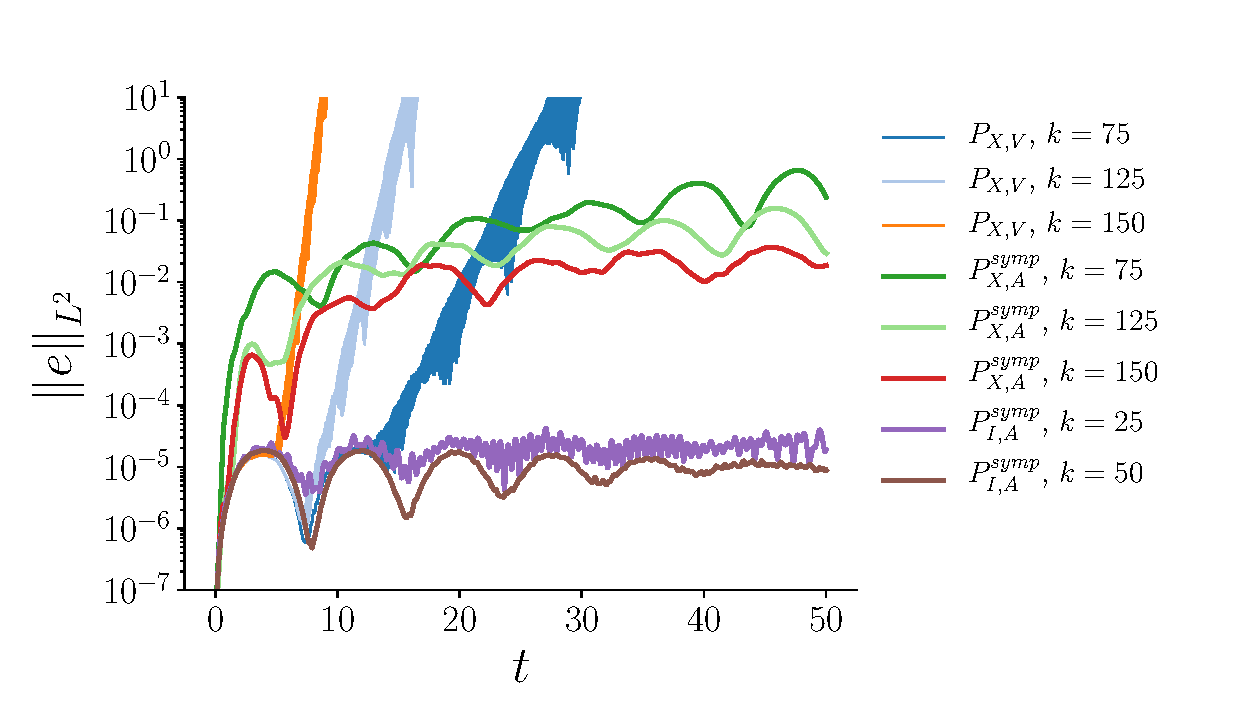
\includegraphics[width=0.45\textwidth]{./figs/beam/l2_norm} & 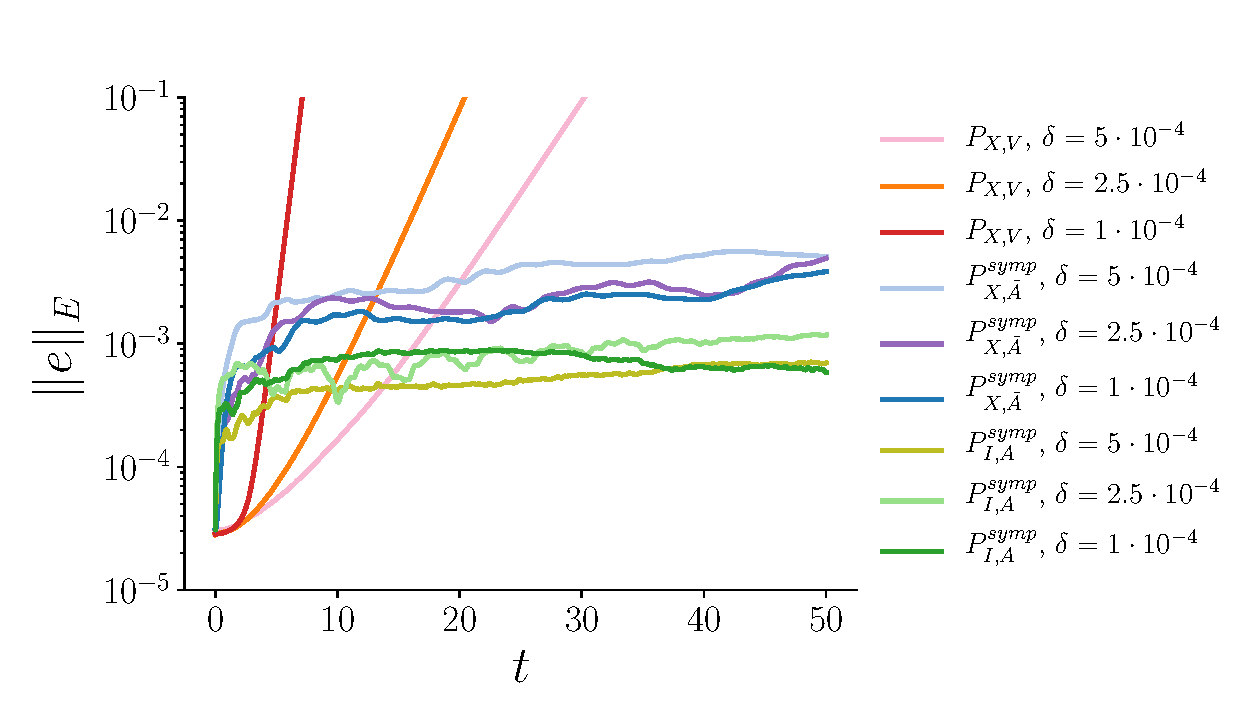
\includegraphics[width=0.45\textwidth]{./figs/beam/energy_norm} \\
(c) & (d) \\
\end{tabular}
\caption{(a) the decay of the singular values. (b) conservation of the Hamiltonian. (c) error with respect to the $L^2$ norm. (d) error with respect to the $X$-norm.}
\end{figure}

Figure \ref{fig:1}a show the decay of the singular values of the time snapshots $S$ and $X^{1/2}S$ respectively. We notice that the decay of the two matrices are different and as the matter of fact the decay saturates for $X^{1/2}S$.

Figure \ref{fig:1}b shows the conservation of the Hamiltonian for all methods mentioned above. It is observed that the symplectic methods do preserve the Hamiltonian and system energy. However, the Hamiltonian blows up for the reduced system constructed by the projection $P_{X,V}$. It is also noticeable that as the basis $V$ gets larger, the Hamiltonian blows up faster.

Figure \ref{fig:1}c shows the $L^2$ error of the reduced system generated by the projection. We notice that the reduced system obtained by the non-symplectic method is unstable. It is known that classical reduce basis methods generally become exceedingly unstable as the reduced basis is enriched. This can also be observed here as the reduced system constructed by $P_{X,V}$ is more unstable as $k$ increases. On the other hand, symplectic methods yield a stable reduced system. As the matter of fact, even as the system constructed by the projection $P^{\text{symp}}_{X,A}$ is not based on the $L^2$ projection, the error remains bounded with respect to the $L^2$ norm. 

Figure \ref{fig:1}d also indicates that classical model reduction methods based on the projection $P_{X,V}$ does not necessarily yield a stable reduced system. However, the symplectic methods provide a stable reduced system under long time-integration. We observe that the original symplectic also provide an accurate solution with respect to the $X$-norm. Nevertheless, the relation between the two norms are not generally known and in general depends on problem set up and initial and boundary conditions \cite{DEPARIS20094359}.

\subsection{The Sine-Gordon Equation} \label{sec:res.2}
The sine-Gordon equation arise in differential geometry and quantum physics \cite{Misumi2015}. This equation is a nonlinear generalization of the linear wave equation, given as
\begin{equation} \label{eq:res.12}
\left\{
\begin{aligned}
	u_{t}(t,x) &= v, \quad x\in \Gamma\\
	v_t(t,x) &= u_{xx} - \sin(u), \\
	u(t,0) &= 0 \\
	u(t,1) &= 1
\end{aligned}
\right.
\end{equation}
Here, $x\in \Gamma$ is an one dimensional box of length $L$, $u,v: \Gamma \to \mathbb R$ are scalar functions. The Hamiltonian associated to (\ref{eq:res.12}) is
\begin{equation} \label{eq:res.13}
	H(q,p) = \int_{\Gamma} \frac 1 2 v^2 + \frac 1 2 u_x^2 + 1 - \cos(u) \ dx.
\end{equation}
One can check that $u_{t} = \delta H / \delta v$ and $v_{t} = - \delta H / \delta u$. The sine-Gordon equation admits the solution solution
\begin{equation} \label{eq:res.14}
	u(t,x) = 4 \text{arctan}\left( \exp ( \pm \frac{x - x_0 - ct}{\sqrt{1-c^2}} ) \right),
\end{equation}
where the plus and minus signs are known as the \emph{kink} and \emph{anti-kink} solutions, respectively. Here $|c|<1$ is the wave speed. We discretize the box into $N$ equi-distant grid point $x_i = i\Delta x$, $i=1,\dots,N$. Furthermore, we use standard finite-differences schemes to discretize (\ref{eq:res.12}) to obtain
\begin{equation}
	\dot z = \mathbb J_{2n} L z + \mathbb J_{2n} g(z) + \mathbb J_{2n} c_b.
\end{equation}
Here $z = (q^T,p^T)^T$, $q(t) = (u(t,x_1),\dots,u(t,x_N))^T$, $p(t) = (v(t,x_1),\dots,v(t,x_N))^T$, $c_b$ is the term corresponding to the boundary conditions and
\begin{equation}
	L = 
	\begin{pmatrix}
		Dx^TDx & 0_N \\
		0_N & I_n
	\end{pmatrix}, 
	\quad
	g(z) = 
	\begin{pmatrix}
	\sin(q) \\
	\vec 0
	\end{pmatrix},
\end{equation}
where $Dx$ is the standard matrix differentiation operator. The discrete Hamiltonian, then takes the form
\begin{equation}
	H_{\Delta x} = \Delta x \cdot \frac 1 2 \| p \|^2 + \Delta x \cdot \| D_x q \|^2 + \sum_{i=1}^{N} \Delta x \cdot ( 1 - \cos(q_i) ).
\end{equation}
The system parameters can be found in the table below.
\vspace{0.5cm}
\begin{center}
\begin{tabular}{|l|l|}
\hline
Domain legnth & box: $L = 50$ \\
No. grid points & $n = 250$ \\
Time discretization size & $\Delta t = 0.01$ \\
Wave speed & $c=0.2$ \\
\hline
\end{tabular}
\end{center}
\vspace{0.5cm}

The St\"ormer-Verlet Scheme is used to integrate (\ref{eq:res.12}) in time and generate the snapshot matrix $S$. Similar to the previous subsection, projection operators $P_{X,V}$, $P^{\text{symp}}_{I,A}$ and $P^{\text{symp}}_{X,A}$ are used to construct a reduced system. To accelerate the evaluation of the nonlinear term, the symplectic methods discussed in section (\ref{eq:mor.1}) and (\ref{eq:mor.2}) are coupled with the projection operators $P^{\text{symp}}_{I,A}$ and $P^{\text{symp}}_{X,A}$, respectively. Furthermore, the DEIM approximation is used for efficient evaluation of the reduced system obtained by the projection $P_{X,V}$. The time-stepping scheme used to integrate the reduced systems are taken identical to the ones in section (\ref{sec:res.1})

\section{Conclusion} \label{sec:conc}
We present a model reduction routine that combines the classic model reduction method, defined with respect to a weighted inner product, with symplectic model reduction. This allows the reduced system to be defined with respect to the norms and inner-products that are natural to the problem. Furthermore, the symplectic nature of the reduced system preserves the Hamiltonian structure of the original system, which results in robustness and enhanced stability in the reduced system.

We demonstrate that including the weighted inner-product in the symplectic model reduction can be viewed as a natural extension of the unweighted symplectic method. Therefore, the stability preserving properties of the symplectic method generalize naturally to the new method.

Numerical results suggest that classic model reduction methods with respect to a weighted inner product can help with the boundedness of the system. However, only the symplectic treatment can consistently increase the accuracy of the reduced system. This is consistent with the fact the symplectic methods preserve the Hamiltonian structure.

We also show that to accelerate the evaluation of the nonlinear terms, adopting a symplectic approach is essential. This allows an accurate reduced model that is consistently enhanced when the basis for the nonlinear term is enriched.

Hence, the symplectic model-reduction with respect to a weighted inner product can provide an accurate and robust reduced system that allows the use of the norms and inner products most appropriate to the problem.

\section*{Acknowledgments} We would like to show our sincere appreciation to Dr. Claudia Maria Colciago for the several brainstorming meetings which helped with the development of the main parts of this article. We would also like to thank Prof. Karen Willcox for hosting Babak Maboudi Afkham at MIT during the composition of this paper. 


\bibliographystyle{siamplain}
\bibliography{references}

\end{document}
